\documentclass{article}

\title{Zarządzanie i harmonogramowanie procesów - zadanie 2}
\author{Artur Dziedziczak 315900}
\date{\today}

\usepackage{subcaption}
\usepackage{microtype}
\usepackage[
    backend=biber,
    natbib=true,
    url=true,
    doi=true,
    eprint=false
]{biblatex}
\usepackage[a4paper, total={6in, 8in}]{geometry}

\addbibresource{sample.bib}
\usepackage{gensymb}
\usepackage{graphicx}

\usepackage{hyperref}
\hypersetup{
    colorlinks=true,
    linkcolor=blue,
    filecolor=magenta,
    urlcolor=cyan,
    pdftitle={Zarządzanie i harmonogramowanie procesów - Zad. 1 Artur Dziedziczak 315900},
    pdfpagemode=FullScreen,
    }

\usepackage{float}

\usepackage[utf8]{inputenc}
\usepackage{amsthm}
\usepackage{enumitem}
\usepackage[english, polish]{babel}
\usepackage[T1]{fontenc}
\usepackage{theorem}
\usepackage{listings}

\lstset{frame=tb,
  language=Bash,
  aboveskip=3mm,
  belowskip=3mm,
  showstringspaces=false,
  columns=flexible,
  basicstyle={\small\ttfamily},
  numbers=none,
  numberstyle=\tiny\color{gray},
  keywordstyle=\color{blue},
  commentstyle=\color{dkgreen},
  stringstyle=\color{mauve},
  breaklines=true,
  breakatwhitespace=true,
  tabsize=3
}

\usepackage[justification=centering]{caption}
\begin{document}

\maketitle

\section {Szeregowanie zadań na jednakowych procesorach równoległych}
\subsection{Zadania podzielne}

Na podstawie podanych danych \(n\) - liczba procesów,
\(p_j\) - czas wykonania \(j\)-tego zadania, określić minimalny czas,
w jakim można zakończyć wszystkie zadania (\(C_{max}\)).
Stworzyć harmonogram realizujący wyznaczony czas.

Przedstawiony problem jest to problem P2|pmtn|Cmax to znaczy problem szeregowania podzielnych i niezależnych zadań na dwóch procesorach z kryterium $C_{max}$.

Można je zamodelować w GLPK w następujący sposób.

\noindent Model matematyczny: \\\\

\noindent Identyfikacja zbiorów:

$T_j$ - zadania do wykonania $j = {A,B,C,D,E,F,G,H}$

$L_{l}$ - procesor na którym wykonywane są zadania $l = {1,2}$

\noindent Parametry modelu:

$p_{jl}$ - czas wymagany do wykonania zadania $p_j$ na procesorze $l$ gdzie $j = {A,B,C,D,E,F,G,H}$, $l = {1,2}$

\noindent Zmienne decyzyjne:

$C_{max}$ - zmienna określająca maksymalny czas pracy maszyny
$x_{jl}$ - czas wykonywania zadania $x_j$ na procesorze $l$ gdzie $j = {A,B,C,D,E,F,G,H}$, $l = {1,2}$

\noindent Funkcja celu:

$min C_{max}$ - maksymalny czas zakończenia

\noindent Ograniczenia:

$\sum{j}{l = 1} x_{jl} = p_j$ - każde zadania jest musi trwać przez podany czas 

$\sum{l}{j = 1} x_{jl} <= C_{max}$ - każda maszyna może pracować przez najwyżej $C_{max}$

$\sum{j}{l = 1} x_{jl} <= C_{max}$ - wartość $C_{max}$ jest najwyższa ze wszystkich czasów przetwarzania $p_j$

\lstinputlisting[
language=AMPL,
numbers=left,
firstnumber=1,
caption={Kod solvera zad1a.mod},
aboveskip=10pt,
]
{glpsol/zad1a.mod}

\lstinputlisting[
language=AMPL,
numbers=left,
firstnumber=1,
caption={Kod wynikowy solvera zad1a.mod},
aboveskip=10pt,
]
{glpsol/zad1a.output}

Jak widać solver znalazł minimalny czas w jaki można zakończyć wszystkie zadania $41$ jednostek czasu.

Dla tego rozwiązania wytworzyłem również harmonogram.

\begin{figure}[h]    
  \centering    
  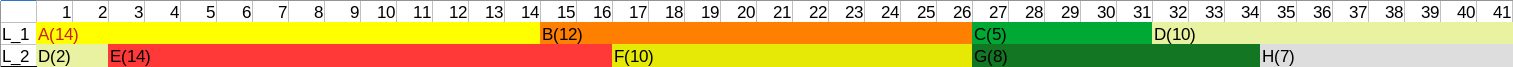
\includegraphics[width=\linewidth]{others/zad1a_harmonogram.png}
  \caption{Harmonogram dla zad1a}
\end{figure}

Jak widać zadanie $D$ zostało podzielone na 2 procesory.

\subsection{Zadania niepodzielne}

\begin{enumerate}[label=(\alph*)]
    \item Mając dane: (n) - liczba procesów, $(p_j)$ - czas wykonania
          $(j)$-tego zadania, stworzyć model minimalizujący czas wykonania
          wszystkich zadań ($(C_{max}$)). Porównać wynik z rozwiązaniem,
          gdy zadania były podzielne.
          Jaka zależność zachodzi w ogólnym przypadku między rozwiązaniami tych zadań?
    \item Zaproponować regułę przydziału zadań minimalizującą czas
          wykonania wszystkich zadań ($(C_{max}$)).
          Porównać wynik z rozwiązaniem optymalnym - jaka zależność zachodzi w ogólnym przypadku?
    \item Mamy Rozwiązanie - niekoniecznie optymalne. Zaproponuj algorytm lokalnej poprawy rozwiązania.
\end{enumerate}


\end{document}
